\documentclass[10pt,a4paper]{article}
\usepackage[latin1]{inputenc}
\usepackage{amsmath}
\usepackage{amsfonts}
\usepackage{amssymb}
\usepackage{graphicx}

\begin{document}
\section{ASSIGNMENT NO: A4}
Author:\:   Ameeth Kanawaday\\
Roll No:\:  4430\\
\section{Problem Definition}
Parser for sample language using YACC.


\section{Learning Objectives:}
\begin{enumerate}
\item To understand the concept of a parser.
\item To use YACC as a parser generator.
\end{enumerate}

\section{S/W and H/W requirements:}
\begin{enumerate}
\item Open source 64 bit OS.
\item Gedit text editor.
\item flex.
\item bison.
\end{enumerate}

\section{Theory}
\textbf{Syntax Analysis:}
\\This is also known as \textbf{Parsing}. t takes the token produced by lexical analysis as input and generates a parse tree (or syntax tree). In this phase, token arrangements are checked against the source code grammar, i.e. the parser checks if the expression made by the tokens is syntactically correct.
\\\\Syntax analyzers follow production rules defined by means of context-free grammar. The way the production rules are implemented (derivation) divides parsing into two types : top-down parsing and bottom-up parsing.
\\\\
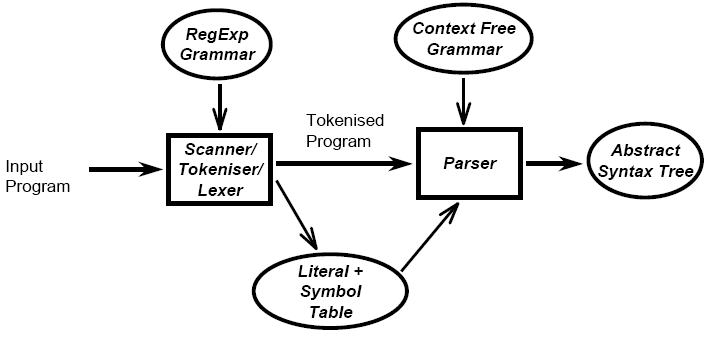
\includegraphics[scale=0.5]{im1.png}
\\\\
\textbf{YACC:}
\\Yacc provides a general tool for imposing structure on the input to a computer program. The Yacc user prepares a specification of the input process; this includes rules describing the input structure, code to be invoked when these rules are recognized, and a low-level routine to do the basic input. Yacc then generates a function to control the input process. This function, called a parser, calls the user-supplied low-level input routine (the lexical analyzer) to pick up the basic items (called tokens) from the input stream. These tokens are organized according to the input structure rules, called grammar rules; when one of these rules has been recognized, then user code supplied for this rule, an action, is invoked; actions have the ability to return values and make use of the values of other actions. 
\\\\Yacc is written in a portable dialect of C[1] and the actions, and output subroutine, are in C as well. Moreover, many of the syntactic conventions of Yacc follow C. 

\section{Related Mathematics}
Let S be the solution perspective of the given problem.
\\The set S is defined as:
\\$S=\lbrace\ s,e,X,Y,F,DD,NDD|\varnothing_{s}\rbrace$
\\Where,
\\s= Start point 
\\e= End point 
\\F= Set of main functions
\\DD= set of deterministic data
\\NDD= set of non deterministic data
\\\\X= Input Set.
\\X = $\lbrace arithematic expression tokens, grammear rules \rbrace$.
\\\\ Y = $\lbrace valid, invalid \rbrace$ 
\\\\ s = available expression.
\\ e = expression verified.
\\\\ F = $\lbrace f_{read}, f_{lex}, f_{match}, f_{ret} \rbrace$
\\\\$f_{read}$  :function to read the expression.
\\\\$f_{lex}$ :function to generate tokens for given arithematic expression.
\\\\ $f_{match}$ :function to match the tokens with grammar rules.
\\\\ $f_{ret}$ :function to return result for expression.
\\\\ DD = $\lbrace tokens, grammar rules \rbrace$
\\ NDD = $\phi$


\section{State Diagram}
\includegraphics[scale=0.5]{cl1a4.png}
\\q0 = read input code state
\\q1 = token generation state
\\q2 = grammar rule matching state
\\q3 = valid expression state
\\q4 = invalid expression state
\\qf = final state

\section{Program}
\begin{verbatim}

////main.l

%{
#include<stdio.h>
#include "y.tab.h"
extern int yylval;
%}

%%
[0-9]+ {
          yylval=atoi(yytext);
          return NUMBER;
       }
[\t] ;
\n return 0;
. return yytext[0];
%%

int yywrap()
{
    return 1;
}


////main.y

%{
    #include<stdio.h>
    int flag=0;
   
%}

%token NUMBER
%left '+' '-'
%left '*' '/' '%'
%left '(' ')'

%%
ArithmeticExpression: E{
         printf("Result = %d ",$$);
         return 0;
        }
//S: SS | DIR 
E:E'+'E {$$=$1+$3;}
 |E'-'E {$$=$1-$3;}
 |E'*'E {$$=$1*$3;}
 |E'/'E {$$=$1/$3;}
 |E'%'E {$$=$1%$3;}
 |'('E')' {$$=$2;}
 | NUMBER {$$=$1;}
;
%%

void main()
{
    printf("\nEnter Any Arithmetic Expression:\n");
    yyparse();
    if(flag == 0)
        printf("\nExpression is Valid.\n\n");
}
void yyerror()
{
    printf("\nExpression is Invalid\n\n");
    flag = 1;
}

OUTPUT:
ameeth@ubuntu-16.0.4:~/Downloads/A4$ lex main.l
ameeth@ubuntu-16.0.4:~/Downloads/A4$ yacc -dv main.y
ameeth@ubuntu-16.0.4:~/Downloads/A4$ gcc lex.yy.c y.tab.c

ameeth@ubuntu-16.0.4:~/Downloads/A4$ ./a.out

Enter Any Arithmetic Expression:
a=b+4

Expression is Invalid

ameeth@ubuntu-16.0.4:~/Downloads/A4$ ./a.out

Enter Any Arithmetic Expression:
5+c

Expression is Invalid

ameeth@ubuntu-16.0.4:~/Downloads/A4$ ./a.out

Enter Any Arithmetic Expression:
5=3+2
Result = 5 
Expression is Valid.

ameeth@ubuntu-16.0.4:~/Downloads/A4$ 



\end{verbatim}
\section{Conclusion}
Thus we successfully implemented YACC program for sample language to check the validity of arithmatic expression.
\end{document}